\tab Ennek a modulnak a feladata az adat (24 bit-es blokkok) adagolása a \textbf{WS2813\_Driver}-nek. Az adagolandó adat BRAM memóriában van tárolva. A modul végzi a címzést.

\tab A \textbf{WS2813\_Driver} modul képes egy 24 bit-es blokk kiküldésére. Ez a modul teszi lehetővé, hogy több 24 bit-es blokk kiküldhető legyen a LED-fűzérre.

\tab A \textbf{WS2813\_Driver} modul egy 24 bit-es blokk elküldése után a \textbf{done} jelét '1'-esre állítja, ezáltal jelzi a felsőbb szintű modulnak, hogy a küldés befejeződött.
Ebben a szekcióban a \textbf{WS2813\_Driver} modul \textbf{done} jelére $Driver_{done}$-ként lesz hivatkozva. A \textbf{done} a controller modul \textbf{done} jelére fog vonatkozni.
Ugyanúgy a \textbf{WS2813\_Driver} modul \textbf{reset}, \textbf{start} $Driver_{reset}$ és $Driver_{start}$ lesznek.

\subsubsection{Elvégzendő RT műveletek azonosítása}

\tab A címzéshez szükséges egy érték dekrementálása. A cím 0-tól 89-ig lehet (90 LED-es ledfűzér). A nullához való hasonlítás hatékonyabb, mint a fix értékhez való,
de ebben az esetben nem ezért volt ez a megoldás felhasználva (max értékről dekrementálás nulláig). 

\tab A BRAM feltöltésekor az az elvárt, hogy az az adat ami a BRAM memóriában a 0-ás címen van, az első LED-en legyen megjelenítve
(első LED-nek számít az ami a legközelebb van az FPGA laphoz). A WS2813 proktoll úgy van definiálva, hogy amint egy új adat érkezik, az összes LED elcsúsztatja a rajta levő értéket jobbra.
Így az az adat ami elsőnek küldődik ki, az utolsó LED-en lesz megjelenítve. Tehát, ha 89-es címen levő adat küldődik ki elsőnek, ez lesz az utolsó LED-en megjelenítve. Értelemszerűen a 0-ás címen
levő adat lesz az első LED-en megjelenítve.

\tab Definiálható RT utasítások: $addr \Leftarrow num\_{leds}$, $addr \Leftarrow addr - 1$

\subsubsection{Adatfüggőségek identifikálása}

\tab Mivel nagyon egyszerű RT műveletekkel meg lehet oldani az adott feladatot, nem merűlnek fel adatfüggőségek.

\subsubsection{Célregiszterek azonosítása}

\tab Szükséges regiszterek:
\begin{itemize}
	\item $R_{addr}$: címet tartalmazó regiszter, a BRAM címzéséhez van felhasználva
\end{itemize}


\subsubsection{Különböző fázisokban elvégzendő műveletek}

\begin{table}[H]
	\begin{center}
		\caption{WS2813\_Controller - Különböző fázisokban elvégzendő műveletek}
		\begin{tabular}{l|c|c|c|c}
		\textbf{Állapot} & $R_{addr}$ 	  & $Driver_{reset}$     & $Driver_{start}$      & done \\
		\hline         
        READY            & $R_{addr}$ 	  & '0'                  & '0'                   & '0'  \\
        \hline         
        INIT             & 89       	  & '0'                  & '0'                   & '0'  \\
        \hline         
        RESET\_DRIVER    & $R_{addr}$  	  & '1'                  & '0'                   & '0'  \\
        \hline         
        START\_DRIVER    & $R_{addr}$  	  & '0'                  & '1'                   & '0'  \\
        \hline         
        SEND             & $R_{addr}$  	  & '0'                  & '0'                   & '0'  \\
        \hline         
		ADDR\_CHECK      & $R_{addr}$     & '0'                  & '0'                   & '0'  \\
        \hline         
        ADDR\_DECR       & $R_{addr} - 1$ & '0'                  & '0'                   & '0'  \\
        \hline         
        FINISHED         & $R_{addr}$     & '0'                  & '0'                   & '1'  \\
		\end{tabular}
	\end{center}
\end{table}


\subsubsection{Kapcsolási rajz}

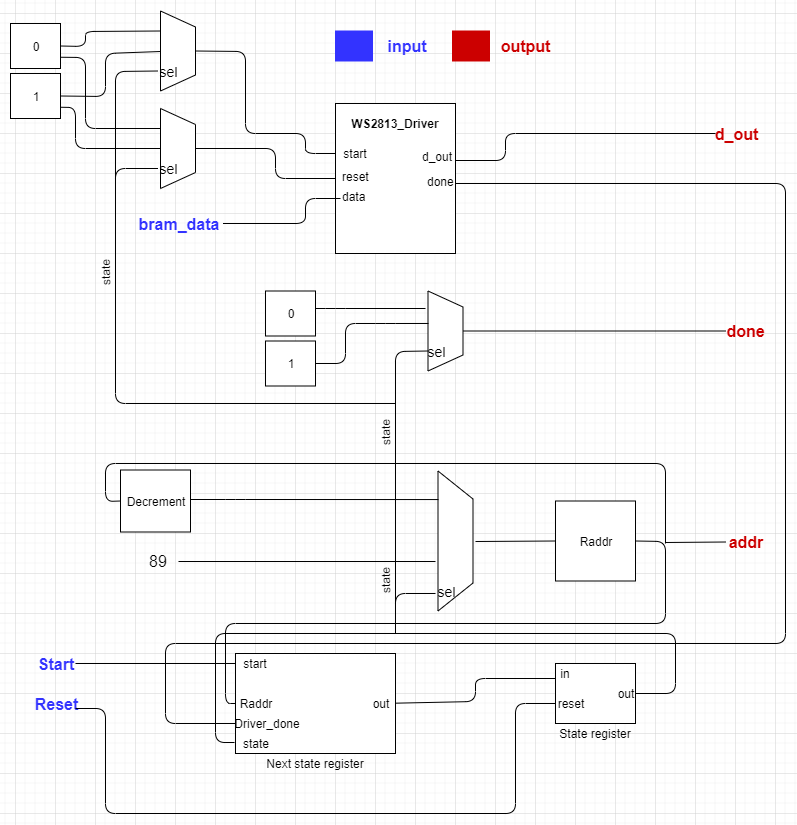
\includegraphics[scale=0.5]{WS2813_Controller_rtl.png}

\subsubsection{Állapotdiagram}

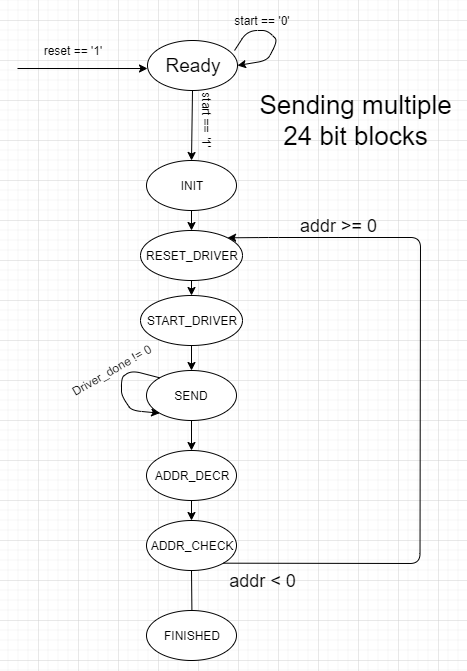
\includegraphics[scale=0.5]{WS2813_Controller_statedia.png}